\chapter{Geodesics in Schwarzschild spacetime}
\label{s:ges}
\index{geodesic!in Schwarzschild spacetime}

\minitoc

\section{Introduction}

We have already investigated some geodesics in Schwarzschild spacetime in
Chap.~\ref{s:sch}, namely
the radial null geodesics (Sec.~\ref{s:sch:rad_null_geod}).
Here, we perform a more extensive study. In particular we investigate timelike
geodesics, which are of primordial physical importance, since they represent
the wordlines of planets or stars orbiting the black hole or of
intrepid observers freely falling into the black hole.

\section{Geodesic motion}

Let $\Li$ be a geodesic\footnote{The definition and basic properties of geodesics
are recalled in Appendix~\ref{s:geo}.} of Schwarzschild spacetime
$(\M,\w{g})$. We shall assume that $\Li$ is causal, i.e. either timelike or null\footnote{As
shown in Sec.~\ref{s:geo:def}, a geodesic cannot be partly timelike and partly
null.}. It therefore can be considered as the worldline
of some particle $\mathscr{P}$, either massive
($\Li$ timelike) or masseless ($\Li$ null).


\subsection{First integrals of motion}

The Schwarzschild spacetime $(\M,\w{g})$ is static and spherically symmetric; the
Killing vector $\w{\xi}$ associated with the staticity (cf. Sec.~\ref{s:sch:static_spher})
and the Killing vector $\w{\eta}$ associated with the rotation symmetry along any
axis, give birth to two conserved quantities along $\Li$:
\begin{greybox}
The scalar products
\begin{subequations}
\label{e:ges:conserved_quantities}
\begin{align}
& \encadre{\veps := - \w{\xi}\cdot \w{p} = - \w{g}(\w{\xi},\w{p}) } \label{e:ges:conserved_energy} \\
& \encadre{\ell := \w{\eta}\cdot \w{p} = \w{g}(\w{\eta},\w{p}) } , \label{e:ges:conserved_angu_mom}
\end{align}
\end{subequations}
where $\w{p}$ is the 4-momentum of particle
$\mathscr{P}$ (cf. Sec.~\ref{s:fra:worldlines}),
are constant along the geodesic $\Li$.
The scalar $\veps$ is called $\mathscr{P}$'s
\defin{conserved energy}\index{conserved!energy}\index{energy!conserved --}
or \defin{energy at infinity}\index{energy!at infinity},
while $\ell$ is called $\mathscr{P}$'s \defin{conserved angular momentum}\index{conserved!angular momuntum}\index{angular momentum!conserved --}
or \defin{angular momentum at infinity}\index{angular momentum!at infinity}.
\end{greybox}
\begin{proof}
The 4-momentum $\w{p}$ is a tangent vector associated with an affine parameter
of $\Li$, i.e. it obeys the geodesic equation (\ref{e:fra:p_geodesic}).
The constancy of $\veps$ and $\ell$ follow then from the generic property (\ref{e:geo:g_xi_v_const})
of geodesics in presence of a spacetime symmetry.
\end{proof}
In coordinates $(t,r,\th,\ph)$ adapted to the spacetime symmetries,
i.e. coordinates such that $\w{\xi} = \wpar_t$ and $\w{\eta}=\wpar_\ph$, like the Schwarzschild-Droste
coordinates or the Eddington-Finkelstein ones, one can rewrite
(\ref{e:ges:conserved_quantities})
in terms of the components $p_t = g_{t\mu} \, p^\mu$ and $p_\ph = g_{\ph\mu} \, p^\mu$
of the 1-form associated to $\w{p}$ by metric duality:
\begin{subequations}
\begin{align}
& \veps = - p_t \\
& \ell = p_\ph
\end{align}
\end{subequations}
Indeed, in such a coordinate system, $\veps = -g_{\mu\nu} \, \xi^\mu p^\nu = -g_{\mu\nu}\,  \delta^\mu_{\ \, t} \, p^\nu = -g_{t\nu} \, p^\nu = -p_t$
and $\ell = g_{\mu\nu} \, \eta^\mu p^\nu = g_{\mu\nu}\,  \delta^\mu_{\ \, \ph} \, p^\nu = g_{\ph\nu} \, p^\nu = p_\ph$.


It is worth stressing that $\veps$ is not a genuine energy, i.e. it is not
an energy measured by some observer. Indeed the latter is defined by
Eq.~(\ref{e:fra:E_obs}), which ressembles Eq.~(\ref{e:ges:conserved_energy})
but differs from it since $\w{\xi}$ is not a unit vector in general:
$\w{\xi}\cdot\w{\xi} \not = -1$. In other words, $\w{\xi}$ cannot in general
be interpreted as the 4-velocity of some observer, thereby making
$\veps$, as defined by (\ref{e:ges:conserved_energy}), fail to be a measured
particle energy. It is only in the asymptotic region, where $\w{\xi}\cdot\w{\xi} = g_{tt}
\rightarrow -1$, that $\w{\xi}$ is an eligible 4-velocity, hence the name
\emph{energy at infinity}. Note that this name is commonly used, even in the
particle $\mathscr{P}$ never visit the asymptotic region.
Similarly, $\ell$ is not some (component of) genuine angular momentum. Only in the
asymptotic region do we have
\be \label{e:ges:ell_asympt}
    \ell \simeq g_{\ph\ph} \, p^\ph \simeq r^2\sin^2\ph \, p^\ph \simeq r^2\sin^2\theta \, P^\ph
    \simeq r\sin\th \, P^{(\ph)} ,
\ee
where $P^{(\ph)}$ is the azimuthal component of the momentum $\w{P}$ of particle $\mathscr{P}$
as measured by an asymptotic inertial observer (cf. Sec.~\ref{s:fra:measure}), i.e.
the component of $\w{P}$ along $\w{e}_{(\ph)}$ in the orthonormal basis $(\w{e}_{(r)}, \w{e}_{(\th)}, \w{e}_{(\ph)})$, with $\w{e}_{(\ph)} = (r\sin\th)^{-1} \wpar_\ph$.
In view of (\ref{e:ges:ell_asympt}), we may say that $\ell$ is the angular momentum
about the symmetry axis $\th=0$ that an inertial observer would attribute to
particle $\mathscr{P}$ if the latter would move close to him.

From its very definition, Eq.~(\ref{e:ges:conserved_energy}), $\veps$ has to be
a positive
quantity as soon as the geodesic $\Li$ has some part in $\M_{\rm I}$, i.e.
some part with $r>2m$:
\begin{greybox}
\be \label{e:ges:eps_positive_M_I}
    \Li \cap \M_{\rm I} \not= \varnothing \quad \Longrightarrow \quad \veps > 0 .
\ee
\end{greybox}
\begin{proof}
In $\M_{\rm I}$, the Killing vector $\w{\xi}$ is timelike and future-directed.
The 4-momentum $\w{p}$ is either timelike or null and always future-directed.
By Eq.~(\ref{e:fra:scalar_caus1}), one has then necessarily $\w{\xi}\cdot\w{p} < 0$; hence Eq.~(\ref{e:ges:conserved_energy})
implies $\veps > 0$ in $\M_{\rm I}$. Since $\veps$ is constant along $\Li$, it
follows that $\veps > 0$ everywhere.
\end{proof}
\begin{remark}
If the geodesic $\Li$ is confined to $\M_{\rm II}$, i.e. to the black hole
region (cf. Sec.~\ref{s:sch:BH}),
where $\w{\xi}$ is spacelike (cf. Sec.~\ref{s:sch:SD_domain}),
it is possible to have $\veps \leq 0$, since the
scalar product of $\w{p}$ with a spacelike vector can take any value.
\end{remark}
\begin{remark}
Since the Killing vector $\w{\eta}$ is always spacelike, there is no constraint
on the sign of $\ell$.
\end{remark}

To be specific, let us describe Schwarzschild spacetime in terms of the
Schwarzschild-Droste coordinates $(t,r,\th,\ph)$ introduced in Sec.~\ref{s:sch:solving_EE}.
Without any loss of generality, we may choose these coordinates such that
at $t=0$, the particle $\mathscr{P}$ is located in the equatorial plane $\th=\pi/2$ and
the spatial projection of the worldline $\Li$ lies in that plane, i.e. $\w{p}$ has
no component along $\wpar_\th$:
\be
    \w{p} \stackrel{t=0}{=} p^t \wpar_{t} + p^r \wpar_r + p^\ph \wpar_\ph .
\ee
Now, if for $t>0$, the geodesic $\Li$ were departing from $\th=\pi/2$, this
would constitute some breaking of spherical symmetry, making a difference
between the ``Northern'' hemisphere and the ``Southern'' one. Hence $\Li$
must stay at $\th=\pi/2$, which implies
\be \label{e:ges:pth_zero}
    \encadre{p^\th = 0} .
\ee
We conclude that
\begin{greybox}
A geodesic $\Li$ of Schwarzschild spacetime is necessarily confined to a timelike hypersurface.
Without any loss of generality, we can choose Schwarzschild-Droste coordinates $(t,r,\th,\ph)$
such that this hypersurface is the ``equatorial hyperplane'' $\th=\pi/2$.
Then the component $p^\th$ of the 4-momentum of the particle having $\Li$ as worldline
vanishes identically [Eq.~(\ref{e:ges:pth_zero})].
\end{greybox}

Let us denote by $\mu$ the mass of particle $\mathscr{P}$, with possibly
$\mu=0$ if $\mathscr{P}$ is a photon. The scalar square of the 4-momentum $\w{p}$ is
then [cf. Eq.~(\ref{e:fra:def_mass})]
\be \label{e:ges:p2_mu2}
    \w{g}(\w{p},\w{p}) = - \mu^2 .
\ee

\subsection{Equations to be solved}

Contemplating Eqs.~(\ref{e:ges:conserved_energy}), (\ref{e:ges:conserved_angu_mom}),
(\ref{e:ges:pth_zero}) and (\ref{e:ges:p2_mu2}), we realize that we have
four first integral of motions. The problem is then completely integrable.
More specifically, let $\lambda$ be the affine parameter along the geodesic
$\Li$ associated with the 4-momentum $\w{p}$ (cf. Eq.~(\ref{e:geo:v_dxdlambda}):
\be
    \w{p} = \frac{\D\w{x}}{\D\lambda} .
\ee
In terms of the components with respect to Schwarzschild-Droste coordinates,
this yields
\be \label{e:ges:comp_4_momentum}
    \dot{t} := \frac{\D t}{\D\lambda} = p^t,\qquad
    \dot{r} := \frac{\D r}{\D\lambda} = p^r,\qquad
    \dot{\th} := \frac{\D \th}{\D\lambda} = p^\th,\qquad
    \dot{\ph} := \frac{\D \ph}{\D\lambda} = p^\ph .
\ee
In the present case, where $\th(\lambda)=\pi/2$, we have of course $\dot{\th}=0$,
in agreement with Eq.~(\ref{e:ges:pth_zero}).
Given the components (\ref{e:sch:Schwarz_metric_SD}) of Schwarzschild metric
with respect to the Schwarzschild-Droste coordinates,
Eq.~(\ref{e:ges:conserved_energy}) can be written as
\[
    \veps = - g_{t\mu} p^\mu = - g_{tt} p^t = - g_{tt} \dot{t}
    = \left(1 - \frac{2m}{r} \right) \dot{t} ,
\]
hence
\be \label{e:ges:dot_t}
    \encadre{\frac{\D t}{\D \lambda} = \veps \left(1 - \frac{2m}{r} \right) ^{-1} }.
\ee
Similarly, Eq.~(\ref{e:ges:conserved_angu_mom}) becomes
\[
    \ell = g_{\ph\mu} p^\mu = g_{\ph\ph} p^\ph  = g_{\ph\ph} \dot{\ph}
        = r^2 \sin^2\th \, \dot{\ph} .
\]
Since $\th=\pi/2$, we get
\be \label{e:ges:dot_ph}
    \encadre{\frac{\D\ph}{\D\lambda} = \frac{\ell}{r^2} } .
\ee
The last unexploited first integral of motion is Eq.~(\ref{e:ges:p2_mu2}); it
yields
\[
   - \left( 1 - \frac{2m}{r} \right) (\dot{t})^2 +
   \left( 1 - \frac{2m}{r} \right) ^{-1}  (\dot{r})^2
   + r^2 (\dot{\th})^2 + r^2 \sin^2\th (\dot{\ph})^2  = - \mu^2 .
\]
Using (\ref{e:ges:dot_t}), (\ref{e:ges:dot_ph}), as well as
$\dot{\th}=0$ and $\th=\pi/2$, we get
\[
    -  \veps^2 \left(1 - \frac{2m}{r} \right) ^{-1}
    +  \left( 1 - \frac{2m}{r} \right) ^{-1}  (\dot{r})^2
    +  \frac{\ell^2}{r^2} = - \mu^2 ,
\]
which can be recast as
\be \label{e:ges:dot_r_square}
    \encadre{ \left( \frac{\D r}{\D \lambda} \right) ^2
        - \frac{2 \mu^2 m}{r} + \frac{\ell^2}{r^2}
         \left( 1 - \frac{2m}{r} \right) = \veps^2 - \mu^2 } .
\ee
To summarize, we may say that the geodesic motion in Schwarzschild spacetime is governed by
Eqs.~(\ref{e:ges:dot_t}), (\ref{e:ges:dot_ph}) and (\ref{e:ges:dot_r_square}),
where $r=r(\lambda)$ and $\mu$, $\veps$ and $\ell$ are constants.
This constitutes a system of 3 differential equations for the 3 unknown
functions $t(\lambda)$, $r(\lambda)$ and $\ph(\lambda)$.
We observe
that Eq.~(\ref{e:ges:dot_r_square}) is decoupled from the other two equations.
The task is then to first solve this equation for $r(\lambda)$ and to inject
the solution into Eqs.~(\ref{e:ges:dot_t}) and (\ref{e:ges:dot_ph}), which
can then be integrated separately.

A constraint to keep in mind is that the 4-momentum vector $\w{p}$, whose
components are related to the solution $(t(\lambda), r(\lambda), \ph(\lambda))$
by Eq.~(\ref{e:ges:comp_4_momentum}), has to be a future-directed causal vector.
In $\M_{\rm I}$, as we have seen above, this is guaranteed by choosing $\veps > 0$
[cf. Eq.~(\ref{e:ges:eps_positive_M_I})]. In $\M_{\rm II}$, a future-directed
timelike vector is $-\wpar_r$ (cf. Sec.~\ref{s:sch:time_orientation}).
According to Eq.~(\ref{e:fra:scalar_caus1}), we have then
$\w{p}$ future-directed iff $-\wpar_r\cdot\w{p} < 0$, i.e. iff
\[
    \left(\frac{2m}{r} - 1  \right) ^{-1} p^r < 0  .
\]
Since $2m/r - 1 > 0$ in $\M_{\rm II}$, this is equivalent to $p^r < 0$, i.e.
to $\D r/\D\lambda < 0$. Hence
\begin{greybox}
In the black hole region $\M_{\rm II}$, i.e. for $r<2m$,
the solution $r(\lambda)$ of Eq.~(\ref{e:ges:dot_r_square})
must be a strictly decreasing function of $\lambda$.
\end{greybox}
Actually, we recover the result stated for any causal worldline (not necessarily
a geodesic) in Sec.~\ref{s:sch:time_orientation}.

\begin{remark}
We have derived the system of Eqs.~(\ref{e:ges:dot_t}), (\ref{e:ges:dot_ph}) and (\ref{e:ges:dot_r_square}) without invoking explicitly the
famous \emph{geodesic equation}\index{geodesic!equation}\index{equation!geodesic --}, i.e.
Eq.~(\ref{e:geo:eq_geod}) in Appendix~\ref{s:geo}.
This is because we had enough
first integrals of that second-order differential equation to completely reduce it to
a system of first order equations.
\end{remark}

In what follows, we discuss separately the resolution of
Eq.~(\ref{e:ges:dot_r_square}) for timelike geodesics and for null ones.


\section{Timelike geodesics}

\subsection{Effective potential}

When the geodesic $\Li$ is timelike, it is natural to use the proper time $\tau$
as an affine parameter along it, instead to the parameter $\lambda$ associated
with the 4-momentum $\w{p}$. Since the tangent vector associated with $\tau$
is the 4-velocity $\w{u}$ (cf. Sec.~\ref{s:fra:massive_part}) and $\w{p}$ and $\w{u}$ are related by
Eq.~(\ref{e:fra:p_m_u}): $\w{p} = \mu \, \w{u}$, we get
$\D\w{x}/\D\lambda = \mu \, \D\w{x}/\D\tau$, from which we infer the relation
between $\tau$ and $\lambda$:
\be
    \tau = \mu \lambda ,
\ee
which of course a special case of the generic relation (\ref{e:geo:affine_transf})
between two affine parameters of the same geodesic.
Equation~(\ref{e:ges:dot_r_square}) becomes then
\be \label{e:ges:1d_motion_timelike}
    \encadre{ \frac{1}{2} \left( \frac{\D r}{\D \tau} \right) ^2
        + V_{\rm eff}(r) = \frac{\bar{\veps}^2 - 1}{2} } ,
\ee
with
\be \label{e:ges:V_eff_timelike}
     \encadre{V_{\rm eff}(r) := - \frac{m}{r} + \frac{\bar{\ell}^2}{2 r^2}
     - \frac{\bar{\ell}^2 m}{r^3} }
\ee
and
\be
   \bar{\veps} := \frac{\veps}{\mu} \qquad\mbox{and}\qquad
   \bar{\ell} :=  \frac{\ell}{\mu} .
\ee
We notice that Eq.~(\ref{e:ges:1d_motion_timelike}) takes the shape of
the 1-dimensional motion of a non-relativist particle in the potential
$V_{\rm eff}$, the term $1/2 \, (\D r/\D\tau)^2$ being interpreted as
the kinetic energy per unit mass, $V_{\rm eff}(r)$ as the potential
energy per unit mass and the constant right-hand side $(\bar{\veps}^2-1)/2$ as the total
mechanical energy per unit mass.

The profile  of $V_{\rm eff}(r)$ for selected values of $\bar{\ell}$ is
plotted in Figs.~\ref{f:ges:eff_pot} and \ref{f:ges:eff_pot_zoom} .
Its extrema are given by
$\D V_{\rm eff}/\D r=0$, which is equivalent to
\[
    m r^2 - \bar{\ell}^2 r + 3 \bar{\ell}^2 m = 0 .
\]
This quadratic equation admits real roots iff $|\bar{\ell}| \geq \bar{\ell}_{\rm crit}$
with
\be \label{e:ges:ell_crit}
   \encadre{ \bar{\ell}_{\rm crit} = 2\sqrt{3} m }.
\ee
For $|\bar{\ell}| \geq \bar{\ell}_{\rm crit}$, the two roots are
\be
    r_{\rm max} = \frac{\bar{\ell}}{2m} \left( \bar{\ell} -
    \sqrt{\bar{\ell}^2 - \bar{\ell}_{\rm crit}^2} \right)
    \qquad\mbox{and}\qquad
    r_{\rm min} = \frac{\bar{\ell}}{2m} \left( \bar{\ell} +
    \sqrt{\bar{\ell}^2 - \bar{\ell}_{\rm crit}^2} \right) ,
\ee
corresponding respectively to a maximum of $V_{\rm eff}$ and a minimum
of $V_{\rm eff}$, hence the indices ``max'' and ``min''. Note that
$r_{\rm max} \leq r_{\rm min}$.
In the marginal case $|\bar{\ell}| = \bar{\ell}_{\rm crit}$, the two roots
coincide and correspond to an inflection point of $V_{\rm eff}$ (the circled
dot in Fig.~\ref{f:ges:eff_pot_zoom}).

For $|\bar{\ell}| < \bar{\ell}_{\rm crit}$, there is no extremum and
$V_{\rm eff}$ is a scritly increasing function of $r$.

\begin{figure}
\centerline{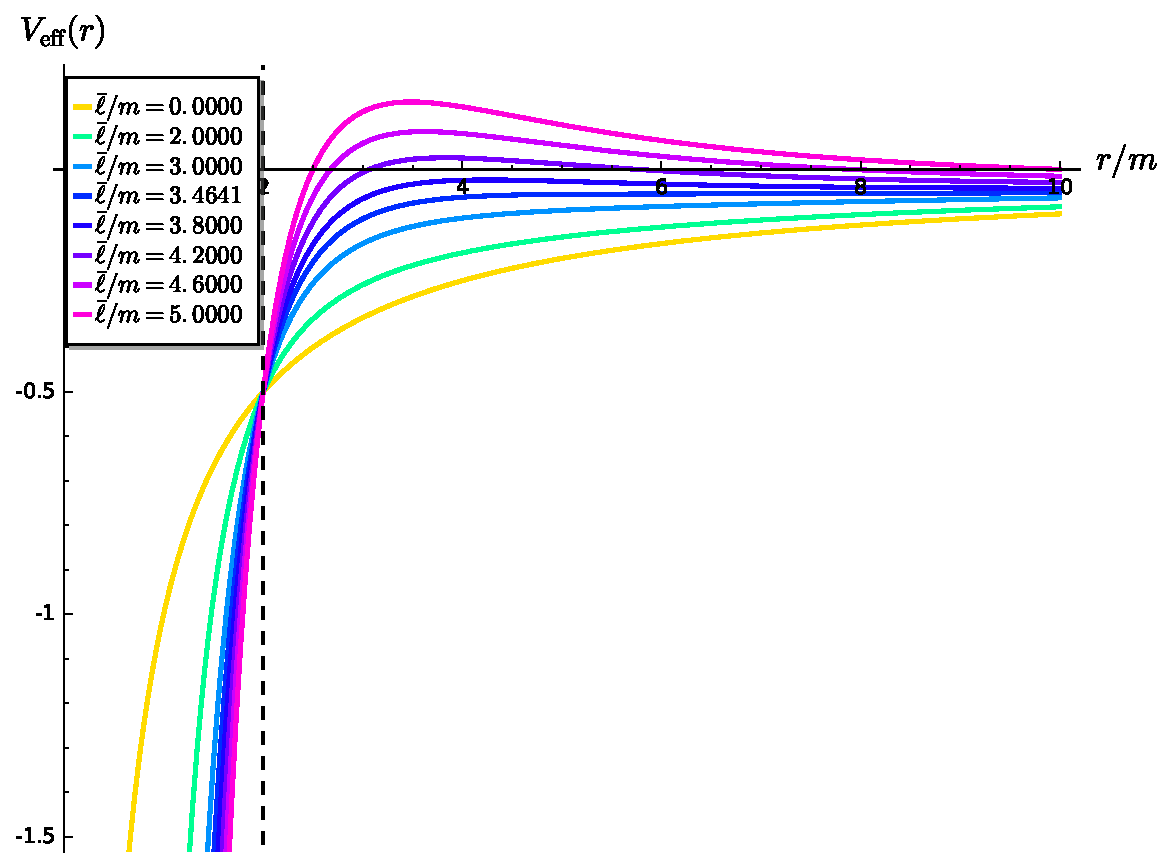
\includegraphics[width=0.8\textwidth]{ges_eff_pot.pdf}}
\caption[]{\label{f:ges:eff_pot} \footnotesize
Effective potential ruling the radial motion along a timelike geodesic in
Schwarzschild spacetime. The vertical dashed line marks $r=2m$, i.e. the
location of the event horizon.
The numerical value $\bar{\ell}/m=3.4641$ is that of the critical
specific angular momentum (\ref{e:ges:ell_crit}).}
\end{figure}

\begin{figure}
\centerline{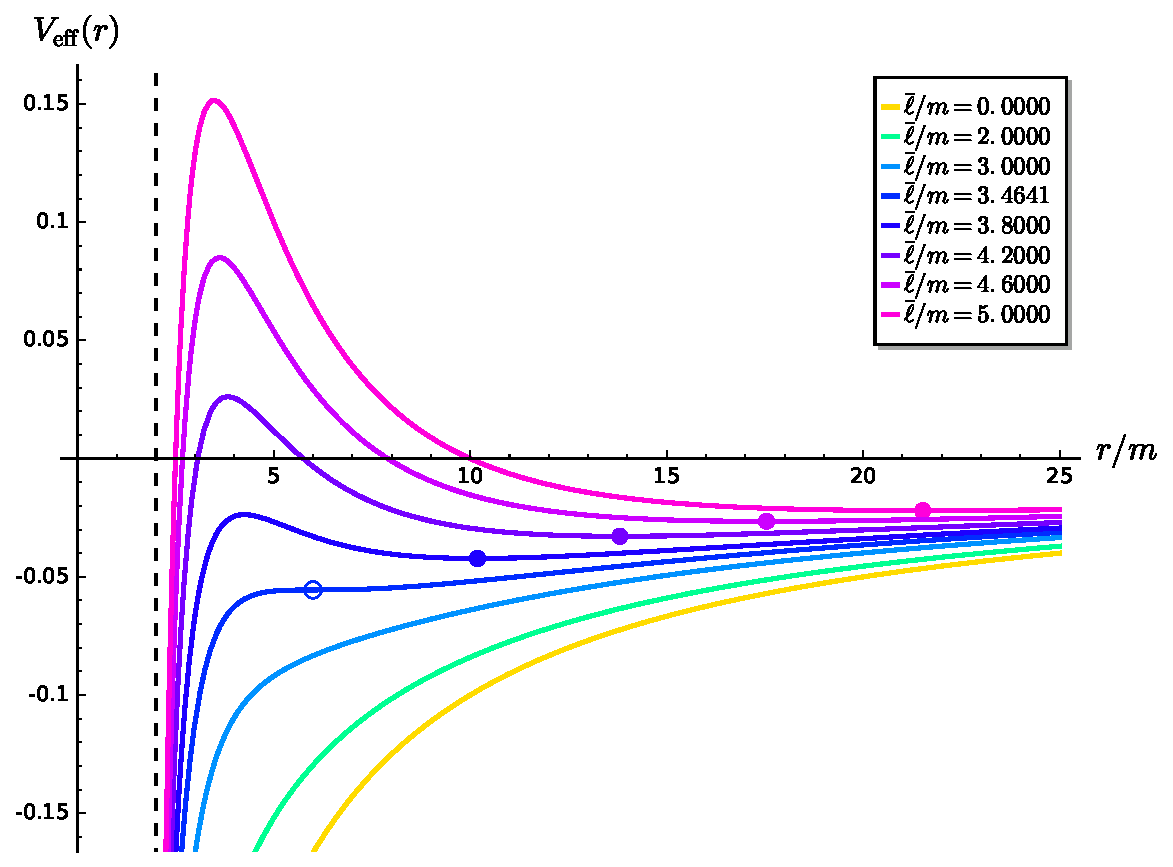
\includegraphics[width=0.8\textwidth]{ges_eff_pot_zoom.pdf}}
\caption[]{\label{f:ges:eff_pot_zoom} \footnotesize
Same as Fig.~\ref{f:ges:eff_pot}, but with a zoom in along the $y$-axis
and a zoom out along the $x$-axis. The dots mark the mimima of
$V_{\rm eff}$, locating stable circular orbits.}
\end{figure}

To get a full solution in terms of the Schwarzschild-Droste coordinates,
once Eq.~(\ref{e:ges:1d_motion_timelike}) is solved for $r(\tau)$,
one has still to solve Eqs.~(\ref{e:ges:dot_t}) and (\ref{e:ges:dot_ph}),
which can be rewritten in terms of the proper time $\tau$ as
\be \label{e:ges:Dt_Dtau}
    \frac{\D t}{\D \tau} = \bar{\veps} \left(1 - \frac{2m}{r(\tau)} \right) ^{-1} ,
\ee
\be
    \frac{\D\ph}{\D\tau} = \frac{\bar{\ell}}{r(\tau)^2}  .
\ee


\subsection{Radial free fall} \label{s:ges:radial_free_fall}

The radial geodesics correspond to a vanishing conserved angular momentum:
$\ell = 0$. Indeed, setting $\ell=0$ in Eq.~(\ref{e:ges:dot_ph}) yields
$\ph = \mathrm{const}$, which defines a pure radial trajectory in the
plane $\th=\pi/2$.
The effective potential (\ref{e:ges:V_eff_timelike}) reduces then
to $V_{\rm eff}(r) = - m/r$, so that the equation of radial motion
(\ref{e:ges:1d_motion_timelike}) becomes
\be \label{e:ges:radial_motion}
    \frac{1}{2} \left( \frac{\D r}{\D \tau} \right) ^2
        - \frac{m}{r} = \frac{\bar{\veps}^2 - 1}{2} .
\ee
As it is well known, the solution of this equation
depends on the sign of the ``mechanical energy'' in the right-hand
side, i.e. of the position of $\bar{\veps}$ with respect to $1$, or
equivalently of that of the conserved energy $\veps$ with respect
to the particle's mass $\mu$:
\begin{itemize}
\item if $\veps>\mu$, the solution
is given in parametrized form (parameter $\eta$) by
\be \label{e:ges:sol_E_pos}
    \left\{ \begin{array}{l}
    \displaystyle\tau = \frac{m}{(\bar{\veps}^2 - 1)^{3/2}} \left( \sinh\eta - \eta \right)
        + \tau_0 \\[2ex]
    \displaystyle r = \frac{m}{\bar{\veps}^2 - 1} \left( \cosh\eta - 1 \right),
    \end{array} \right.
\ee
\item if $\veps=\mu$, the solution is
\be \label{e:ge:sol_E_zero}
    r(\tau) =  \left( \frac{9 m}{2} (\tau -\tau_0)^2 \right) ^{1/3} ,
\ee
\item if $\veps<\mu$, the solution
is given in parametrized form (parameter $\eta$) by
\be \label{e:ges:sol_E_neg}
    \left\{ \begin{array}{l}
    \displaystyle\tau =  \frac{m}{|\bar{\veps}^2 - 1| ^{3/2}} \left( \eta + \sin\eta \right)
    + \tau_0  \\[2ex]
    \displaystyle r = \frac{m}{|\bar{\veps}^2 - 1|} \left( 1 + \cos\eta \right),
    \end{array} \right.
\ee
\end{itemize}
In the above formulas, $\tau_0$ is a constant; for $\veps\geq \mu$,
it sets the value of $\tau$ for which $r\rightarrow 0$, while
for $\veps<\mu$, it sets the value of $\tau$ at which $r$ takes its maximal value.

Let consider the concrete case of a radial free-fall from rest, starting at some
position $r=r_0$ at $\tau=0$. Assuming a departure from rest
means $\D r/\D\tau = 0$ at $\tau=0$. The equation of radial motion
(\ref{e:ges:radial_motion}) leads then to $-m/r_0 = (\bar{\veps}^2 - 1)/2$,
or equivalently
\be \label{e:ges:beps2}
         \bar{\veps}^2 = 1 - \frac{2m}{r_0} .
\ee
The right-hand side of this equation must be non-negative. This implies
$r_0\geq 2m$. We recover the fact that one cannot be momentarily at rest
(in terms of $r$) if $r_0<2m$, for $r$ has to decrease along any future-directed
worldline in the black hole region $\M_{\rm II}$ (cf. Sec.~\ref{s:sch:time_orientation}).

Equation~(\ref{e:ges:beps2}) implies $\bar{\veps} < 1$, i.e. $\veps < \mu$. The solution
is thus given by Eq.~(\ref{e:ges:sol_E_neg}); expressing $|\bar{\veps}^2 - 1|$
via (\ref{e:ges:beps2}), we get
\be \label{e:ges:sol_radial_infall}
    \encadre{
    \left\{ \begin{array}{l}
    \displaystyle\tau = \sqrt{\frac{r_0^3}{8 m}}  \left( \eta + \sin\eta \right) \\[3ex]
    \displaystyle r = \frac{r_0}{2} \left( 1 + \cos\eta \right)
    \end{array} \right. }
    \qquad 0 \leq \eta \leq \pi ,
\ee
where the range of $\eta$ is such that $r=r_0$ for $\tau=0$ ($\eta=0$) and
$r$ decays to $0$ when $\eta\rightarrow \pi$.
The solution for $t=t(\tau)$ is obtained by combining $\D t/\D\tau$ as expressed
by (\ref{e:ges:Dt_Dtau}) and $\D\tau/\D\eta$ deduced from (\ref{e:ges:sol_radial_infall}):
\[
    \frac{\D\tau}{\D\eta} = \sqrt{\frac{r_0^3}{8 m}}  \left( 1 + \cos\eta \right)
        = \sqrt{\frac{r_0}{2m}} \, r .
\]
We get
\[
    \frac{\D t}{\D\eta} =  \frac{\D t}{\D\tau} \frac{\D\tau}{\D\eta}
        = \bar{\veps} \sqrt{\frac{r_0}{2m}} \, r \left(1 - \frac{2m}{r} \right) ^{-1}
        = \sqrt{\frac{r_0}{2m} - 1} \; \frac{r^2}{r - 2m} ,
\]
where we have used (\ref{e:ges:beps2}) and $\bar{\veps} > 0$ to write
$\bar{\veps} = \sqrt{1-2m/r_0}$.
Substituting $r$ from Eq.~(\ref{e:ges:sol_radial_infall}), we get
\[
    \frac{\D t}{\D\eta} =   \frac{r_0}{2} \sqrt{\frac{r_0}{2m} - 1} \;
        \frac{(1+\cos\eta)^2}{1+\cos\eta - 4m/r_0} .
\]
This equation can be integrated to
\be \label{e:ges:sol_t_radial_infall}
   \encadre{ t = 2m \left\{ \sqrt{\frac{r_0}{2m} - 1} \left[ \eta + \frac{r_0}{4m}
    (\eta + \sin\eta) \right]
    + \ln \left| \frac{\sqrt{\frac{r_0}{2m} - 1} + \tan\frac{\eta}{2}}{\sqrt{\frac{r_0}{2m} - 1} - \tan\frac{\eta}{2}} \right| \right\} } ,
\ee
where we have assumed $t=0$ at $\tau=0$ ($\eta=0$).

The solution of the radial free fall starting from rest at $r=r_0$ is
thus given in parametric form by Eqs.~(\ref{e:ges:sol_radial_infall}) and
(\ref{e:ges:sol_t_radial_infall}). It has been obtained in the Schwarzschild-Droste coordinates
$(t,r,\th,\ph)$, which are singular at the event horizon $\Hor$. So, one might wonder
if such a solution can describe the full infall, with the crossing of $\Hor$.
In particular, we notice that the differential equation for $t(\tau)$,
Eq.~(\ref{e:ges:Dt_Dtau}), is singular at $r=2m$, i.e. on $\Hor$. The solution
$t(\eta)$, as given by Eq.~(\ref{e:ges:sol_t_radial_infall}) is singular at
$\eta=\eta_*$, where
\be
    \eta_* := 2 \,\mathrm{atan}\, \sqrt{\frac{r_0}{2m} - 1}
\ee
is precisely the value of $\eta$ yielding $r=2m$ in Eq.~(\ref{e:ges:sol_radial_infall})
[to see it, rewrite the second part of Eq.~(\ref{e:ges:sol_radial_infall}) as
$r=r_0\cos^2(\eta/2) = r_0/(1+\tan^2(\eta/2))$].

\subsection{Circular orbits}



\section{Null geodesics}


\begin{hist}
Synge \cite{Synge66}, Bardeen \cite{Barde73}
\end{hist}
